\documentclass{article}
\usepackage[utf8]{inputenc}

% \usepackage{multicol}
\usepackage{url}
\usepackage[style=verbose,autocite=footnote]{biblatex}
\usepackage{diagbox}
\usepackage{graphicx}
\usepackage{parskip}

\graphicspath{{img/}}

\bibliography{bibli}

\title{A New Way of looking at the Trigonometric Sign Convention}
\author{Param Siddharth \\ \url{http://www.paramsid.com}}
\date{July 2020}

\renewcommand{\arraystretch}{1.5}

\begin{document}

\maketitle

    \begin{abstract}
        This document talks about a way of looking at the trigonometric sign convention different from the traditional technique, involving lines and triangles in place of the Cartesian plane and circles.
    \end{abstract}
    
    % \vspace*{\fill}
    % \textbf{Keywords} \\
    % Mathematics, Trigonometry, Science, Physics, Geometry

\newpage \vspace*{8cm}
\thispagestyle{empty}
\begin{center}
    \large \emph{Dedicated to}
    
    \emph{My parents, and my brother, who have always had my back.}
\end{center}
\newpage

\tableofcontents
\newpage

\section{Introduction}

Trigonometry is a part of mathematics that encompasses universal aspects of physics. It revolves around the relations between side-lengths and angles of triangles, and its contemporary applications are way beyond mathematical problems and physical concepts. Its beauty is evident to the mathematical aesthete.

It will be hard for me to continue without quoting and highlighting the beauty of trigonometry. I shall therefore continue with the same. This urge of mine terminates at page number \pageref{tldr}.

\subsection{Beautiful Applications of Trigonometry}

Trigonometry obviously holds great importance in the field of mathematics.\autocite{Wiki:1}

\begin{enumerate}
    \item Terms in Fourier series contain the use of the sine and cosine functions.
    $$ f(x)=a_0+\sum_{n=1}^\infty \cos \left( \frac{n\pi}{L} x \right)+\sum_{n=1}^\infty \sin \left( \frac{n\pi}{L} x \right) $$
    \item Trigonometric functions are also applied when statisticians study seasonal periodicities, often represented by Fourier series.
    \item It is used in calculating the heights of buildings and mountains.
\end{enumerate}

In science, especially physics, trigonometry plays a huge role.\autocite{Embibe:1}

\begin{enumerate}
    \item The very process of finding the components of vectors relates to the use of trigonometric ratios.
    \item Dot and cross projects of vectors also involve the use of trigonometric functions.
    \item Simple Harmonic Oscillations (SHMs) and various other physical phenomena are defined by trigonometric ratios.
\end{enumerate}

In addition to everything stated above, trigonometry is used in video games, engineering, navigation technology, et cetera.

\newpage

\section{The Sign Convention}
\label{tldr}

The convention of defining the signs of the trigonometric ratios is shown in table \ref{tab:signcon}.

\begin{table}[!h]
    \centering
    \begin{tabular}{|c|c|c|c|c|}
        \hline
        \backslashbox{Function}{Quadrant} & 1 & 2 & 3 & 4 \\
        \hline
        Sine and Cosecant & $+$ & $+$ & $-$ & $-$ \\
        \hline
        Cosine and Secant & $+$ & $-$ & $-$ & $+$ \\
        \hline
        Tangent and Cotangent & $+$ & $-$ & $+$ & $-$ \\
        \hline
    \end{tabular}
    \caption{The Convention}
    \label{tab:signcon}
\end{table}

\begin{table}[!h]
    \centering
    \begin{tabular}{|c|c|}
        \hline
        Quadrant & Angle Range \\ \hline
        1 & $(0,\frac{\pi}{2})$ \\ \hline
        2 & $(\frac{\pi}{2},\pi)$ \\ \hline
        3 & $(\pi,\frac{3\pi}{2})$ \\ \hline
        4 & $(\frac{3\pi}{2}, 2\pi)$ \\
        \hline
    \end{tabular}
    \caption{Quadrants and Angle Ranges}
    \label{tab:quadvang}
\end{table}

\subsection{The Original Justification}

The word \textbf{trigonometry} contains \textit{trigon}. That reminds us that it is related to triangles. The sign convention, however, involves the use of circles and the Cartesian plane more than triangles and angles to be derived.

\begin{figure}[!h]
    \centering
    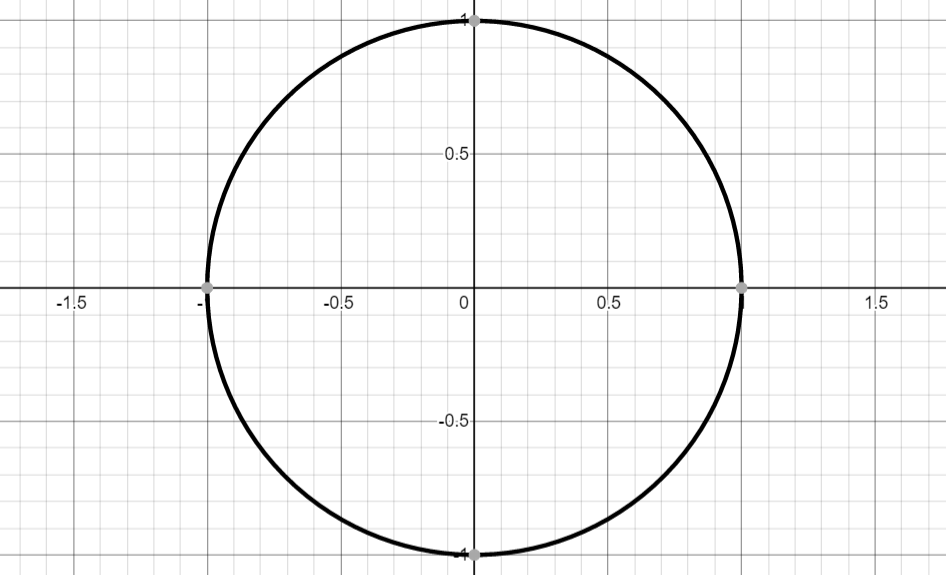
\includegraphics[width=8cm]{circle}
    \caption{A circle in the Cartesian plane}
    \label{fig:circle}
\end{figure}

Figure \ref{fig:circle} contains a circle defined by $x^2+y^2=1$. 

Every point on the circle is represented as $(\cos\theta,\sin\theta)$, where $\theta$ represents the angle between the line segment joining the point on the circle to the origin and the positive $x$-axis, going from the x-axis to the line segment in an anti-clockwise manner. $\cos\theta$ and $\sin\theta$ respectively refer to the $x$ and $y$ co-ordinates of the point (\textit{why?}).

\begin{figure}[!h]
    \centering
    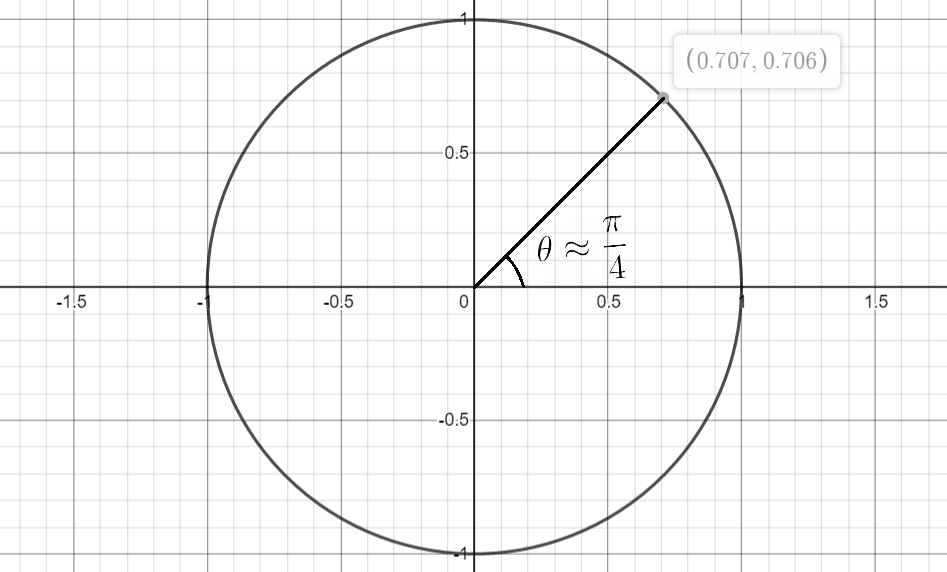
\includegraphics[width=8cm]{circlepoint}
    \caption{A point on the circle}
    \label{fig:circlepoint}
\end{figure}

Figure \ref{fig:circlepoint} shows an example of a point at $\theta\approx\frac{\pi}{4}$ radians.

Since we have defined that this is valid for all points on the circle, it should be valid for all its points that reside in the other quadrants too. In all quadrants excluding quadrant 1, at least one of the co-ordinates is a negative value, which would be used to determine the signs of the trigonometric ratios.

We know that the sign of $\sin\theta$ is the same as that of $\csc\theta$ $\forall$ $\theta$ for which both the functions are defined. The same relation goes for the pairs $\cos$ \& $\sec$, and $\tan$ \& $\cot$, respectively. This observation halves the effort in determining signs, because now we know that 3 pairs of functions will share the same signs each for all the values of the angle each pair is defined for.

Continuing from here, we will talk only about the signs of $\sin$, $\cos$, and $\tan$; The signs of $\csc$, $\sec$, and $\cot$ can be inferred from the same.

\begin{figure}[!h]
    \centering
    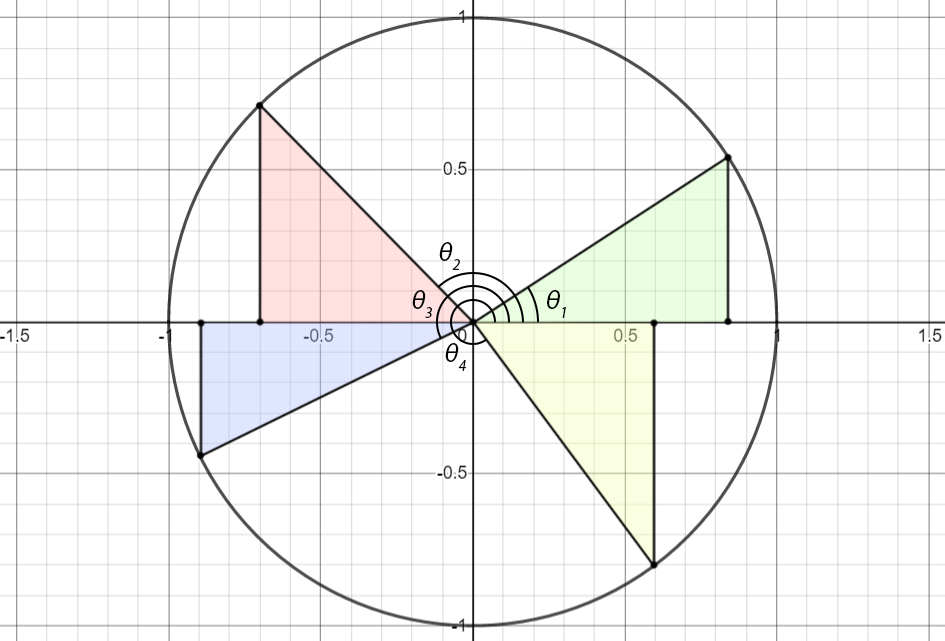
\includegraphics[width=8cm]{circlepoints}
    \caption{Representation of 4 triangles within that circle}
    \label{fig:circlepoints}
\end{figure}

We can see how 4 right-angled triangles are represented in figure \ref{fig:circlepoints}. The points of the triangles meeting the circle can be represented as the aforementioned manner i. e. $(\cos\theta,\sin\theta)$, where $\theta$ represents the angle between the line segment joining that point on the circle to the origin and the positive $x$-axis, going from the x-axis to the line segment in an anti-clockwise manner. Considering that, corresponding to the triangles are angles $\theta_1$, $\theta_2$, $\theta_3$, and $\theta_4$ respectively.

We can easily determine the sign of the $x$ and $y$ co-ordinates of the points by looking at the quadrant they reside in. Also, since $\cos\theta$ and $\sin\theta$ represent the $x$ and $y$ co-ordinates, we can deduce the signs for cosine and sine in the respective angle-ranges. Since the tangent will be the ratio of the sine to the cosine, we can infer its sign too.

Let's start with $\theta_1$. Since the point on the triangle touching the circle resides in quadrant 1, both its $x$ and $y$ co-ordinates will be positive. Hence, we can say that $\cos\theta_1$ and $\sin\theta_1$ will also be positive. Now, since $\theta_1$ lies in quadrant 1, it will be in the range $(0,\frac{\pi}{2})$. We conclude that sine and cosine are positive for the angles in this range. Since the tangent is the ratio of the sine to the cosine, it will also be positive.

Let's look at $\theta_2$ now. It lies in quadrant 2, which tells us that its $x$ co-ordinate is negative and its $y$ co-ordinate is positive. Hence, we can say that $\cos\theta_2$ is negative and $\sin\theta_2$ is positive. $\theta_2$ lies in the range $(\frac{\pi}{2},\pi)$. Hence, for this range, cosine is negative, sine is positive, and tangent is negative (\textit{why?}).

Similarly, we can deduce the convention for the other two angle ranges too. This is the traditional method to derive the sign convention.

\subsection{A Different Way}

Since trigonometry was related to triangles, I believed there ought to be a way to work out the sign convention by using triangles only. In the limited environment I was present in, no textbook or teacher could answer me. \textbf{I was disappointed!} I took a paper and a pencil and set out the search for an answer. The results were terrific.

\begin{figure}[!h]
    \centering
    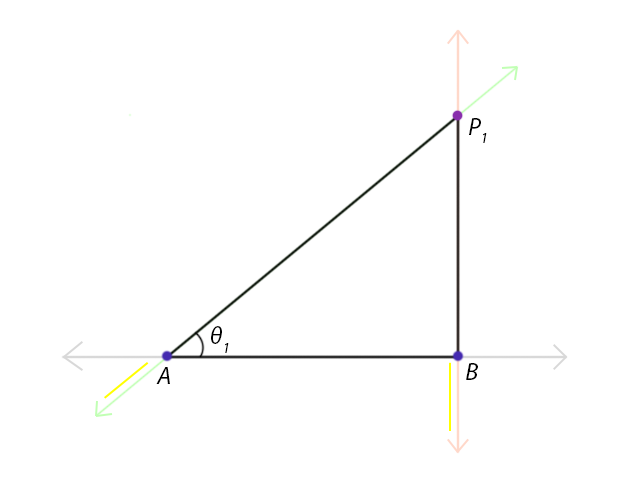
\includegraphics[width=8cm]{triangle1}
    \caption{A right triangle with an angle in range $(0, \frac{\pi}{2})$}
    \label{fig:tri1}
\end{figure}

Figure \ref{fig:tri1} shows the right-angled triangle $\Delta ABP_1$. Lines $AB$, $BP_1$, and $AP_1$ intersect to form the triangle. Points $A$ and $B$ are special; I will refer to them as the pivot points from now on. The grey line passing through $AB$ forms the non-hypotenuse side of the triangle, while the pink line passing through $BP_1$ forms the side opposite to the angle of focus $\theta_1$ here. The green line passing through $AP_1$ forms the hypotenuse. We can freely rotate the green line about the point $A$.

We know that a point lying on a line divides it into 2 rays. Since we are studying the sign convention, we will assign signs to each ray of the 3 lines with respect to the pivot points. 

\begin{itemize}
    \item For the grey line, its ray to the right of $B$ will be negative, and they ray to the left of $B$ will be positive. 
    \item For the pink line, the ray above $B$ will be positive, and the ray below $B$ will be negative. 
    \item For the green line, the ray starting from $A$ going to $P_1$ represents the positive part, while the one going away from $P_1$ represents the negative part.
\end{itemize}

In this analysis, we won't be dealing with the negative ray of the grey line. Therefore, for the pink and green lines only, I will indicate the negative rays with yellow line segments next to them in parallel.

The angle in focus will be represented by $\theta$ with subscripts. $\theta$ will always be the angle between the green and grey lines, starting from the grey line and going in a counter-clockwise fashion. Since the green line is free to rotate about $A$, we can rotate it to alter $\theta$ as well as the intersection point of the green and pink lines, hence generating new triangles. The point of intersection of the green and pink lines will be denoted by $P$ with subscripts.

In figure \ref{fig:tri1}, we will be dealing with $\theta\in(0,\frac{\pi}{2})$. We observe:
$$\sin\theta_1=\frac{BP_1}{AP_1},\ cos\theta_1=\frac{AB}{AP_1},\ \tan\theta_1=\frac{BP_1}{AB}$$
\begin{itemize}
    \item Considering the sine, both $BP_1$ and $AP_1$ lie in the positive rays of the pink and green lines respectively. Hence, their ratio is positive, whereby we conclude that the sine of any angle in the range $(0,\frac{\pi}{2})$ is always positive.
    \item Considering the cosine, both $AB$ and $AP_1$ lie in the positive rays of the grey and green lines respectively. Hence, their ratio is positive, whereby we conclude that the cosine of any angle in the range $(0,\frac{\pi}{2})$ is always positive.
    \item Considering the tangent, both $AB$ and $AP_1$ lie in the positive rays of the pink and grey lines respectively. Hence, their ratio is positive, whereby we conclude that the tangent of any angle in the range $(0,\frac{\pi}{2})$ is always positive.
\end{itemize}

That is it! We have successfully deduced the sign convention for the range $(0,\frac{\pi}{2})$. Let us move on to the range $(\frac{\pi}{2},\pi)$.

\begin{figure}[!h]
    \centering
    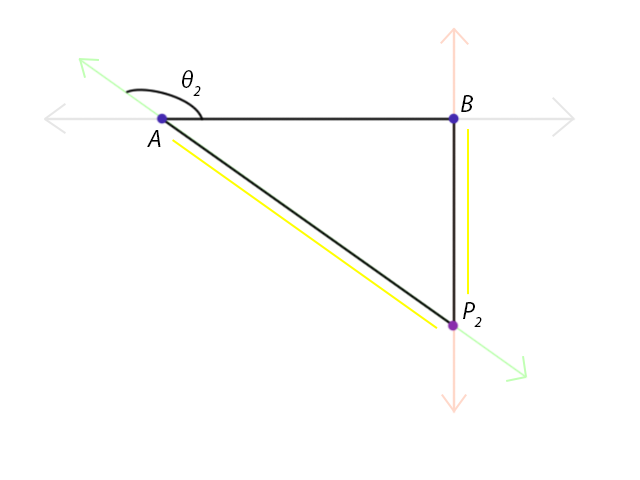
\includegraphics[width=8cm]{triangle2}
    \caption{A right triangle with an angle in range $(\frac{\pi}{2},\pi)$}
    \label{fig:tri2}
\end{figure}

In figure \ref{fig:tri2}, we have rotated the green line about $A$ such that $\theta_2\in(\frac{\pi}{2},\pi)$ and the \emph{negative rays} (indicated by yellow parallel line segments) of the green and pink lines intersect at $P_2$. Our new right-angled triangle is $\Delta ABP_2$. In this triangle, we observe:
$$\sin\theta_2=\frac{BP_2}{AP_2},\ cos\theta_2=\frac{AB}{AP_2},\ \tan\theta_2=\frac{BP_2}{AB}$$
\begin{itemize}
    \item Considering the sine, both $BP_2$ and $AP_2$ lie in the negative rays of the pink and green lines respectively. Hence, their ratio is positive (negative : negative), whereby we conclude that the sine of any angle in the range $(\frac{\pi}{2},\pi)$ is always positive.
    \item Considering the cosine, $AB$ lies in the positive ray of the grey line, while $AP_2$ lies in the negative ray of the green line. Hence, their ratio is negative, whereby we conclude that the cosine of any angle in the range $(\frac{\pi}{2},\pi)$ is always negative.
    \item Considering the tangent, $AB$ lies in the positive ray of the grey line, while $AP_2$ lies in the negative ray of the green line. Hence, their ratio is negative, whereby we conclude that the tangent of any angle in the range $(\frac{\pi}{2},\pi)$ is always negative.
\end{itemize}

And there we did it for quadrant 2 as well. Notice that since the only changing point is $P$ i. e. the intersection of the green and pink lines, the only lines whose participating rays (rays forming the right-angled triangle) may change are the green and pink lines. $AB$ will always be in the positive ray of the grey line for all the 4 quadrants.

\begin{figure}[!h]
    \centering
    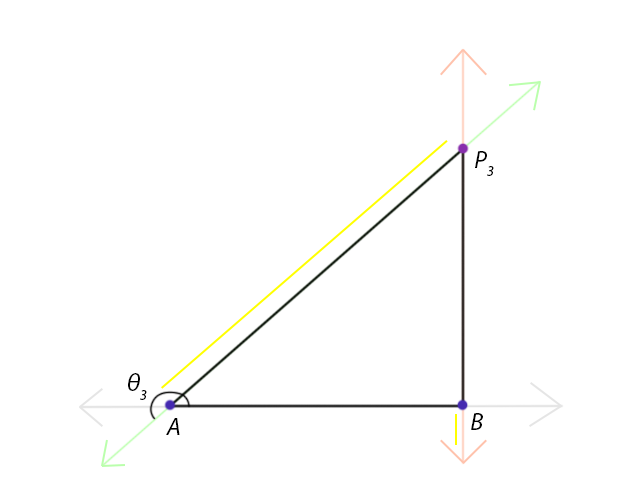
\includegraphics[width=8cm]{triangle3}
    \caption{A right triangle with an angle in range $(\pi,\frac{3\pi}{2})$}
    \label{fig:tri3}
\end{figure}

Figure \ref{fig:tri3} shows a right triangle with $\theta_3\in(\pi,\frac{3\pi}{2})$, which is formed by rotating the green line further anti-clockwise such that its negative ray meets the pink line in its positive ray. In $\Delta ABP_3$, we observe:
$$\sin\theta_3=\frac{BP_3}{AP_3},\ cos\theta_3=\frac{AB}{AP_3},\ \tan\theta_3=\frac{BP_3}{AB}$$
\begin{itemize}
    \item Considering the sine, $BP_3$ lies in the positive ray of the pink line, while $AP_3$ lies in the negative ray of the green line. Hence, their ratio is negative, whereby we conclude that the sine of any angle in the range $(\pi,\frac{3\pi}{2})$ is always negative.
    \item Considering the cosine, $AB$ lies in the positive ray of the grey line, while $AP_3$ lies in the negative ray of the green line. Hence, their ratio is negative, whereby we conclude that the cosine of any angle in the range $(\pi,\frac{3\pi}{2})$ is always negative.
    \item Considering the tangent, both $BP_3$ and $AB$ lie in the positive rays of their respective lines. Hence, their ratio is positive, whereby we conclude that the tangent of any angle in the range $(\pi,\frac{3\pi}{2})$ is always positive.
\end{itemize}

\begin{figure}[!h]
    \centering
    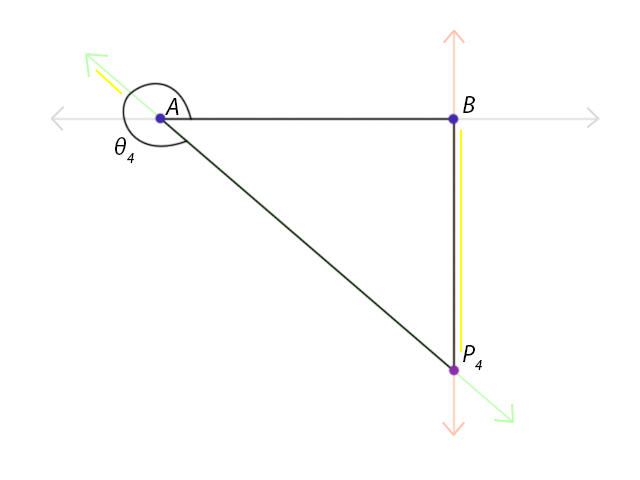
\includegraphics[width=8cm]{triangle4}
    \caption{A right triangle with an angle in range $(\frac{3\pi}{2},2\pi)$}
    \label{fig:tri4}
\end{figure}

Figure \ref{fig:tri4} shows the right triangle $\Delta ABP_4$ generated by rotating the green line such that $\theta_3\in(\frac{3\pi}{2},2\pi)$. The deduction of the sign convention for quadrant 4 is left as an exercise for the reader.

\emph{Quod erat demonstrandum.}

\section{Final Thoughts}

Rediscovering the sign convention by looking at it in a way different from the traditional one was an enlightening experience for me. In "The most unexpected answer to a counting puzzle", Grant Sanderson showed how looking at a mathematical problem from a mathematically aesthetic way can unravel beautiful solutions.\autocite{YouTube:1} Back in 2018, I chose to do the same before I had this wonderful observation.

This non-traditional way of looking at the trigonometric sign convention might not satisfy some readers who prefer the traditional circle technique to deduce it, but I hope it serves as a good means of looking at the convention by involving triangles and angle ranges instead of circles and quadrants. My message to the contemporary youth is that one should continue to question things until they either discover their desired answer or realize they were wrong and accept their defeat. Giving up isn't a choice when you set out to discover something that might have never been discovered before.

\newpage
\printbibliography
\end{document}
